\documentclass[11pt, uplatex, dvipdfmx]{jsarticle}
\usepackage{amsmath,amsfonts, bm, braket, setspace, emathEy, enumitem, graphicx}

\newcommand{\ds}{\displaystyle}
\renewcommand{\dlim}{\lim\limits} %emathEyを使わないなら\newcommand


\resettagform


\pagestyle{plain}



\title{\Huge 線形代数 問題集}


\begin{document}

\maketitle
\thispagestyle{empty}

\newpage

\section{行列}\label{sec:matrix}

\begin{enumerate}[label=\ref{sec:matrix}.\arabic*]
  \setlength{\itemsep}{1zh}
  
\item 次の行列 $A$ に対し,$A^n$ を求めよう.ただし,$n$ は自然数とする.

  \vspace{1ex}
  
  \begin{edaenumerate}<retusuu=3>[(1)]
  \item $A= \left[
      \begin{array}{rr}
        2 & 1\\
        0 & 2
      \end{array}
    \right]$

  \item $A=\left[
      \begin{array}{rrr}
        2 & 1 & 0\\
        0 & 2 & 0\\
        0 & 0 & 3
      \end{array}
    \right]$
    
  \item $A=\left[
      \begin{array}{rrr}
        2 & 1 & 0\\
        0 & 2 & 1\\
        0 & 0 & 2
      \end{array}
    \right]$
  \end{edaenumerate}\vspace{-2zh}

\item $B=\left[
    \begin{array}{rr}
      2 & 1\\
      0 & 2
    \end{array}
  \right], \; P=\left[
    \begin{array}{rr}
      3 & 4\\
      2 & 3
    \end{array}
  \right]$ とする.

  \vspace{1zh}
  
  \begin{enumerate}[label=(\arabic*)]
    \setlength{\itemsep}{1ex}
    
  \item $P^{-1}AP=B$ となる行列 $A$ を求めよう.

  \item 自然数 $n$ に対し,$A^n$ を求めよう.
  \end{enumerate}

\item $A=\left[
    \begin{array}{rr}
      -2 & 2\\
      5 & -3
    \end{array}
  \right]$ とする.

  \vspace{1zh}

  \begin{enumerate}[label=(\arabic*)]
    \setlength{\itemsep}{1ex}
    
  \item $A^2+5A-4E_2$ を計算しよう.

  \item (1) の結果を活用して $A^5$ を効率良く計算しよう.
  \end{enumerate}
  
\item 下図のような $5$ 個の空港 $1, 2, 3, 4 ,5$ を結ぶ航空路線がある.
  空港 $i$ から空港 $j$ への直通路線があるとき $a_{ij}=1$ とし,そうで
  ないとき $a_{ij}=0$ とする.ただし,$a_{ii}=0$ とする.
  \begin{figure}[h]
    \centering
    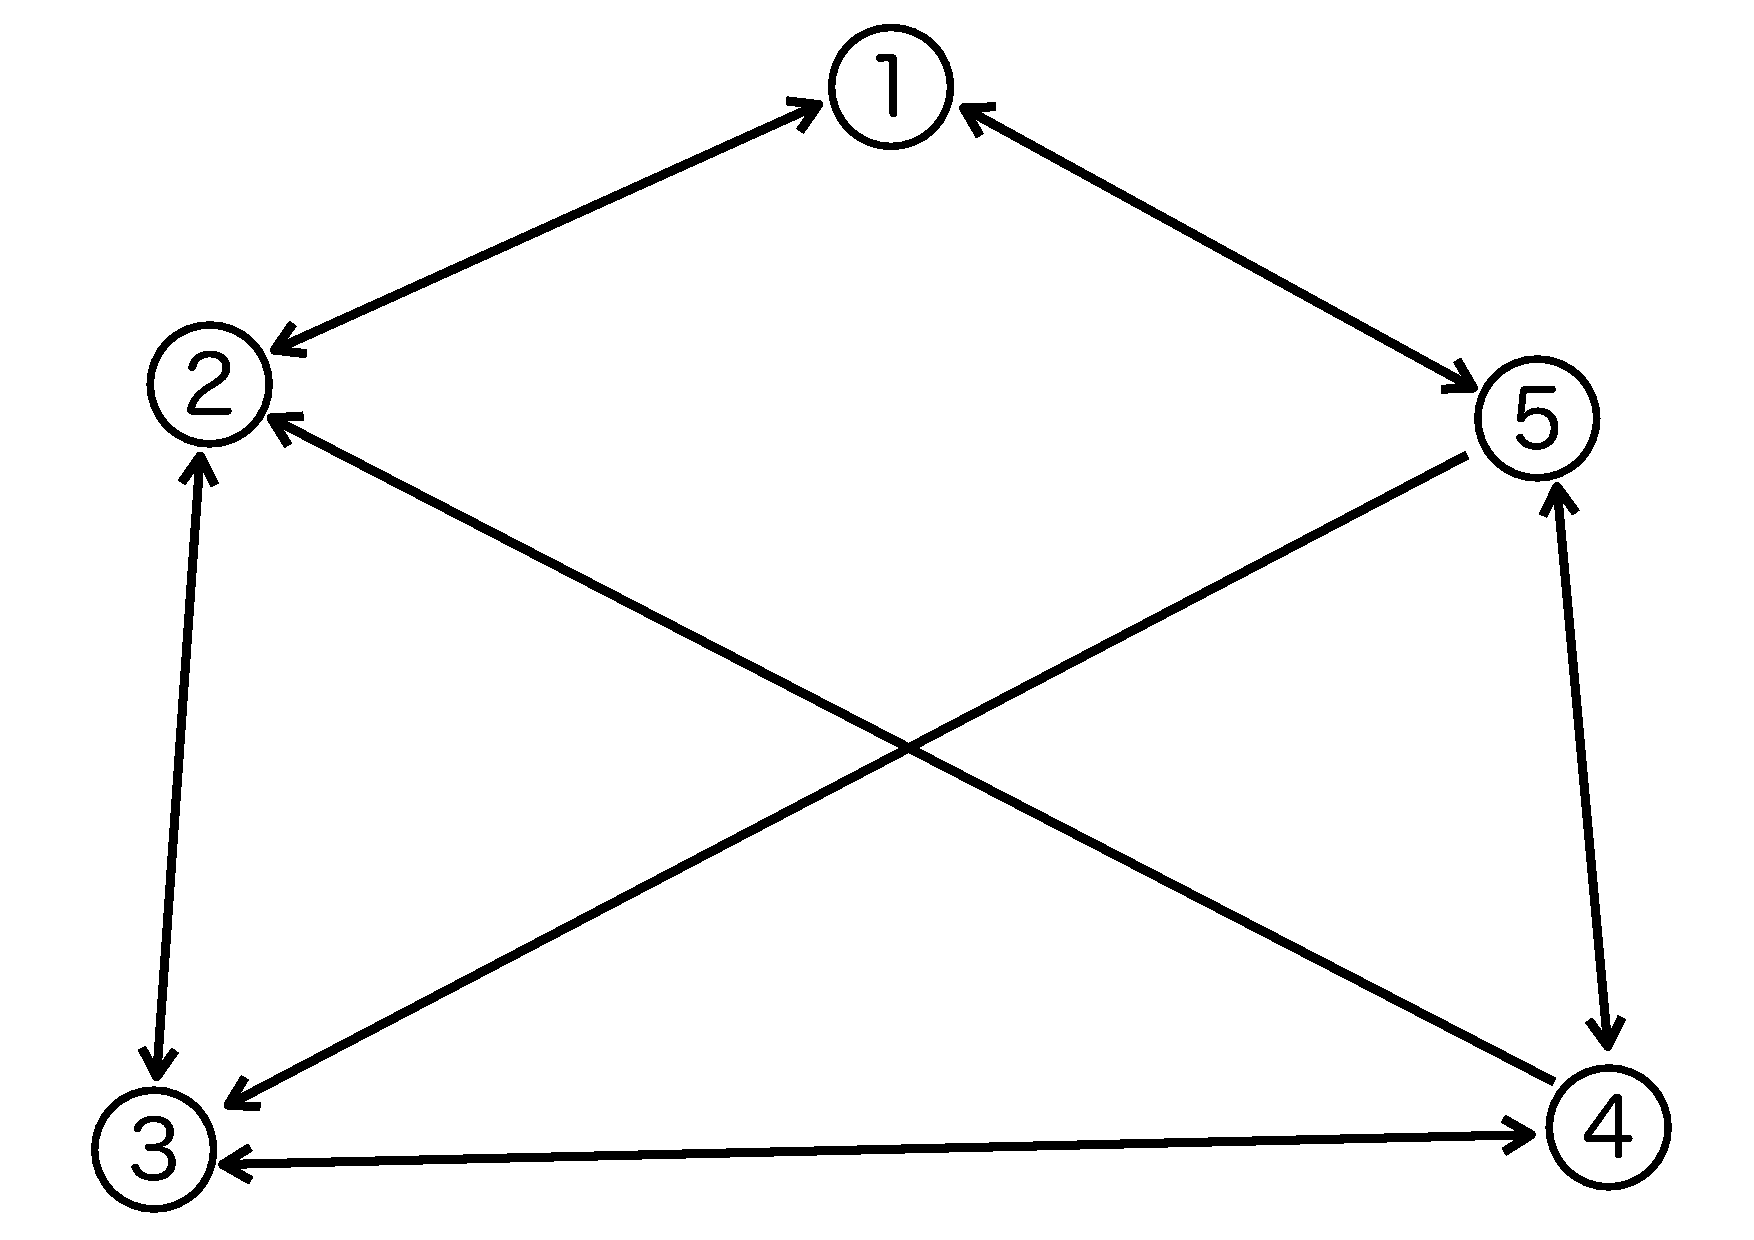
\includegraphics[width=6cm]{./pictures/routes.pdf}
  \end{figure}

  \begin{enumerate}[label=(\arabic*)]
    \setlength{\itemsep}{1ex}
    
  \item $a_{ij}$ を $(i,j)$ 成分とする $5$ 次正方行列 $A=\left[ a_{ij}\right]$ を具体的に書いてみよう.

  \item $A^2, A^3, A^4$ を計算しよう.

  \item $A^2$ の $(i,j)$ 成分は
    $a_{i1} a_{1j} + a_{i2}a_{2j} + a_{i3}a_{3j} + a_{i4}a_{4j} +
    a_{i5}a_{5j}$ であることから,この値が何を意味するか考えよう.

  \item 自然数 $n$ に対して $A^n$ の $(i,j)$ 成分が何を意味するか考えよう.

  \item 路線 $4 \to 2 \to 1 \to 5 \to 3$ のように,空港 $4$ から出発し
    て $4$ 回の移動($3$ 回の乗り継ぎ)で空港 $3$ に到着する路線の個数
    を求めよう.
  \end{enumerate}


\end{enumerate}

% \section{連立1次方程式}\label{sec:system}

% \begin{enumerate}[label=\ref{sec:system}.\arabic*]
%   \setlength{\itemsep}{1zh}
  
% \item 

% \item

% \item
  
% \end{enumerate}

% \section{行列式}\label{sec:determinant}

% \begin{enumerate}[label=\ref{sec:determinant}.\arabic*]
%   \setlength{\itemsep}{1zh}
  
% \item

% \item

% \item
% \end{enumerate}

\end{document}
